%% ============================================================
%%  Classification vs. Retrieval for Trustworthy Skin-Lesion
%%  Screening on Degraded and Real-World Images
%%
%%  IEEE conference format. Compile on Overleaf with the /figures
%%  folder uploaded alongside this file (menu: Recompile).
%%  NOTE: verify all reference details against originals before
%%  formal submission (a few page numbers are approximate).
%% ============================================================
\documentclass[conference]{IEEEtran}
\IEEEoverridecommandlockouts
\usepackage{cite}
\usepackage{amsmath,amssymb,amsfonts}
\usepackage{graphicx}
\usepackage{booktabs}
\usepackage{xcolor}
\usepackage{url}
\usepackage{tikz}
\usetikzlibrary{arrows.meta,positioning}
\usepackage{algorithm}
\usepackage{algpseudocode}
\usepackage[hidelinks]{hyperref}

\begin{document}

\title{Does It Know When It Is Wrong? Classification versus
Retrieval for Trustworthy Skin-Lesion Screening on Degraded and
Real-World Images}

\author{
\IEEEauthorblockN{Nishan Kharel\IEEEauthorrefmark{1} and Paras Simkhadha\IEEEauthorrefmark{2}}
\IEEEauthorblockA{\IEEEauthorrefmark{1}Institute of Science and Technology, Tribhuvan University, Kathmandu, Nepal\\
\IEEEauthorrefmark{2}University of Greenwich, London, United Kingdom\\
Email: nkharel57@gmail.com, simkhadaparash@gmail.com}
}

\maketitle

\begin{abstract}
Deep networks match dermatologists on curated skin-lesion images, yet almost
all are trained and tested on clean, dermatoscopic photographs. In deployment,
especially phone-based screening where a specialist is far away, inputs are
blurry, dark, compressed, or captured with an ordinary camera, and a screening
tool that fails \emph{silently} on them is dangerous. We ask a trust-centred
rather than accuracy-centred question: on degraded and real-world images, which
design is more reliable, a fine-tuned classifier or an embedding-based
case-retrieval model, measured jointly by robustness of the malignant class and
by honesty of its own uncertainty. Using HAM10000 we compare an
EfficientNet-B0 classifier against DINOv2 nearest-neighbour retrieval under a
graded corruption suite and, crucially, on 2{,}106 real smartphone photographs
from PAD-UFES-20 with no retraining, reporting bootstrap 95\% confidence
intervals throughout. Three findings emerge. (i) Aggregate accuracy hides a
melanoma-sensitivity collapse: under low light and noise the classifier's
melanoma recall falls to near zero while retrieval holds at 40--50\%. (ii) A
retrieval model's calibration under distribution shift depends entirely on its
confidence signal---vote share is badly overconfident (ECE 0.23--0.31), whereas
a nearest-neighbour \emph{distance} signal, calibrated on a degraded validation
set, is the best-calibrated of all models even under heavy corruption (ECE
0.03). (iii) On real smartphone photos the retrieval model catches $3.5\times$
more melanomas (0.40 vs.\ 0.115, non-overlapping CIs) and detects that the
images are out-of-distribution (AUROC 0.94 vs.\ 0.72). We also report an honest
negative: confidence-based abstention does not raise melanoma recall, because
calibration and ranking are distinct. Overall accuracy is low for both models
under the real modality shift, as expected; the contribution is that a
retrieval design with the right uncertainty signal is simultaneously more
robust and more honest about what it does not know. Code and data splits are
public.
\end{abstract}

\begin{IEEEkeywords}
skin cancer, melanoma, medical image analysis, robustness, distribution shift,
model calibration, uncertainty estimation, image retrieval, out-of-distribution
detection, trustworthy AI.
\end{IEEEkeywords}

\section{Introduction}
Melanoma is the deadliest common skin cancer and early detection sharply
improves survival. Convolutional networks now rival dermatologists on benchmark
data~\cite{esteva2017}, and public datasets such as HAM10000~\cite{tschandl2018}
and the ISIC challenges~\cite{codella2018} have driven rapid gains. Almost
universally, however, models are trained and evaluated on \emph{clean,
dermatoscopic} images: good optics, even light, the lesion centred and
magnified through a contact lens. The photographs a real person submits, taken
on a phone and often blurry, dark, tilted, or compressed, look nothing like the
training distribution.

This matters because the failure mode is not merely lower accuracy but
\emph{silent} failure: a model that outputs ``benign, 95\% confident'' on a
degraded melanoma actively tells a patient not to seek care. For a screening
tool meant to widen access where dermatologists are scarce, the right question
is therefore not only ``how accurate is it?'' but ``does it know when it is
wrong?''

We study this by comparing two contrasting designs on identical data and
evaluation: a \textbf{classifier} (fine-tuned EfficientNet-B0 mapping an image
to one of seven labels) and a \textbf{retrieval} model (each image embedded by a
frozen DINOv2 network, then classified by a weighted vote over its nearest
stored cases, whose distance to those cases is itself an uncertainty signal). We
evaluate both under a graded corruption suite and under a genuine real-world
shift: real smartphone photographs from PAD-UFES-20~\cite{pacheco2020}, with no
retraining.

\noindent\textbf{Contributions.}
\begin{enumerate}
\item A head-to-head comparison of classification and retrieval for skin-lesion
screening on the axes that matter for trust---robustness of the \emph{malignant}
class and honesty of confidence---rather than clean-set accuracy, with bootstrap
confidence intervals.
\item Evidence that aggregate accuracy \emph{masks} a melanoma-sensitivity
collapse under degradation, visible only when the malignant class is examined
alone.
\item The finding that a retrieval model's calibration under distribution shift
hinges on the confidence signal: a distance-based, shift-calibrated confidence
remains well-calibrated (ECE $\approx0.03$) even under heavy corruption, unlike
vote-share retrieval and the classifier.
\item A real-world validation on smartphone photographs, where retrieval both
catches significantly more melanomas and detects the distribution shift, while
the classifier stays confidently wrong.
\item An honest negative on confidence-based selective prediction, distinguishing
calibration from ranking, plus interpretable case-based error analysis.
\end{enumerate}

\section{Related Work and Gaps}
\subsection{Deep learning for skin-lesion classification}
From dermatologist-level classification~\cite{esteva2017} to standardised
benchmarks~\cite{tschandl2018,codella2018}, accuracy on clean dermoscopy has
risen steadily. Recent foundation models push this further: general
self-supervised features (DINOv2~\cite{oquab2024}), biomedical vision--language
models (BiomedCLIP~\cite{zhang2025biomedclip}), and dermatology-specific models
(PanDerm~\cite{yan2025panderm}). \emph{Gap:} evaluation is almost always on
clean in-distribution test sets, rarely characterising class-specific behaviour
under input degradation.

\subsection{Robustness and distribution shift}
Common-corruption robustness was formalised for natural
images~\cite{hendrycks2019} and adapted to dermoscopy: a dedicated skin-cancer
robustness benchmark~\cite{maron2021}, corruption suites with test-time
adaptation~\cite{hu2024diffusion}, artifact-driven domain
generalisation~\cite{bissoto2022artifact}, and modality-aware corruption
benchmarks including a dermatology split~\cite{disalvo2024medmnistc}.
\emph{Gap:} results are reported as aggregate accuracy, obscuring class-specific
clinical risk such as missed melanomas, and rarely compared across model
paradigms.

\subsection{Calibration and uncertainty}
Modern networks are miscalibrated~\cite{guo2017}; ECE~\cite{naeini2015} and
post-hoc methods such as isotonic regression~\cite{zadrozny2002} quantify and
correct this. In medical imaging, calibration has been studied for skin-lesion
uncertainty and conformal prediction~\cite{fayyad2024conformal}, calibration
robust to label noise~\cite{penso2024calibration}, and the drivers of
calibration across regimes~\cite{sambyal2023understanding}. \emph{Gap:}
calibration is typically assessed in-distribution, and obtaining an honest
confidence for a \emph{retrieval} model under shift is unexplored.

\subsection{Retrieval and case-based diagnosis}
Content-based image retrieval and $k$-nearest-neighbour classification over deep
embeddings offer transparency: saliency-enhanced CBIR for dermatology reader
studies~\cite{gassner2023secbir}, nearest-neighbour search on pretrained medical
features~\cite{gupta2023mednn}, and metric-learning embeddings for
dermoscopy~\cite{he2022demal}. \emph{Gap:} retrieval is seldom pitched
head-to-head against a fine-tuned classifier as a \emph{trustworthiness}
strategy, jointly on robustness and calibration.

\subsection{Out-of-distribution detection}
Maximum softmax probability is the classic OOD baseline~\cite{hendrycks2017}.
Medical OOD benchmarks include MOOD~\cite{zimmerer2022mood} and
OpenMIBOOD~\cite{gutbrod2025openmibood}, with dermatology-specific
detectors~\cite{huang2022multiscale}; dataset-quality studies also document the
leakage and duplication that make honest shift evaluation
hard~\cite{abhishek2025dermamnist}. \emph{Gap:} real cross-dataset OOD in
dermatology (clean dermoscopy training vs.\ real smartphone deployment) and
retrieval distance as the OOD signal are largely untested.

\subsection{Selective prediction and deferral}
Selective classification abstains on low-confidence inputs~\cite{geifman2017};
in clinical AI, learning-to-defer with uncertainty~\cite{liu2022ldu}, calibrated
deferral to multiple experts~\cite{verma2023multiexpert}, and
complementarity-driven deferral~\cite{dvijotham2023codoc} route hard cases to
clinicians. \emph{Gap:} whether a well-calibrated confidence also \emph{ranks}
errors well enough to abstain usefully is rarely tested per-class.

\smallskip
\noindent\textbf{Summary of the gap.} Prior work advances accuracy, robustness,
calibration, retrieval, OOD detection, and deferral largely in isolation and on
clean data. We unify them into one trust-centred evaluation for skin-lesion
screening, with class-specific (melanoma) robustness and real smartphone
validation.

\section{Datasets}
\textbf{HAM10000}~\cite{tschandl2018} has 10{,}015 dermatoscopic images over
seven classes (nv, mel, bkl, bcc, akiec, vasc, df), is 67\% nevi, and is over
half histopathologically confirmed. As the 10{,}015 images come from only
7{,}470 lesions, we split \emph{by lesion} (stratified by diagnosis) into
6{,}981 train / 1{,}532 validation / 1{,}502 test, so no lesion appears in two
splits. \textbf{PAD-UFES-20}~\cite{pacheco2020} has 2{,}298 \emph{smartphone}
clinical images under varied lighting; mapping its labels to the shared classes
(BCC$\rightarrow$bcc, MEL$\rightarrow$mel, NEV$\rightarrow$nv, ACK$\rightarrow$akiec,
SEK$\rightarrow$bkl) and dropping SCC leaves 2{,}106 images. PAD is macroscopic,
a different modality from dermoscopy---a genuine, hard shift.

\begin{figure}[t]
\centering
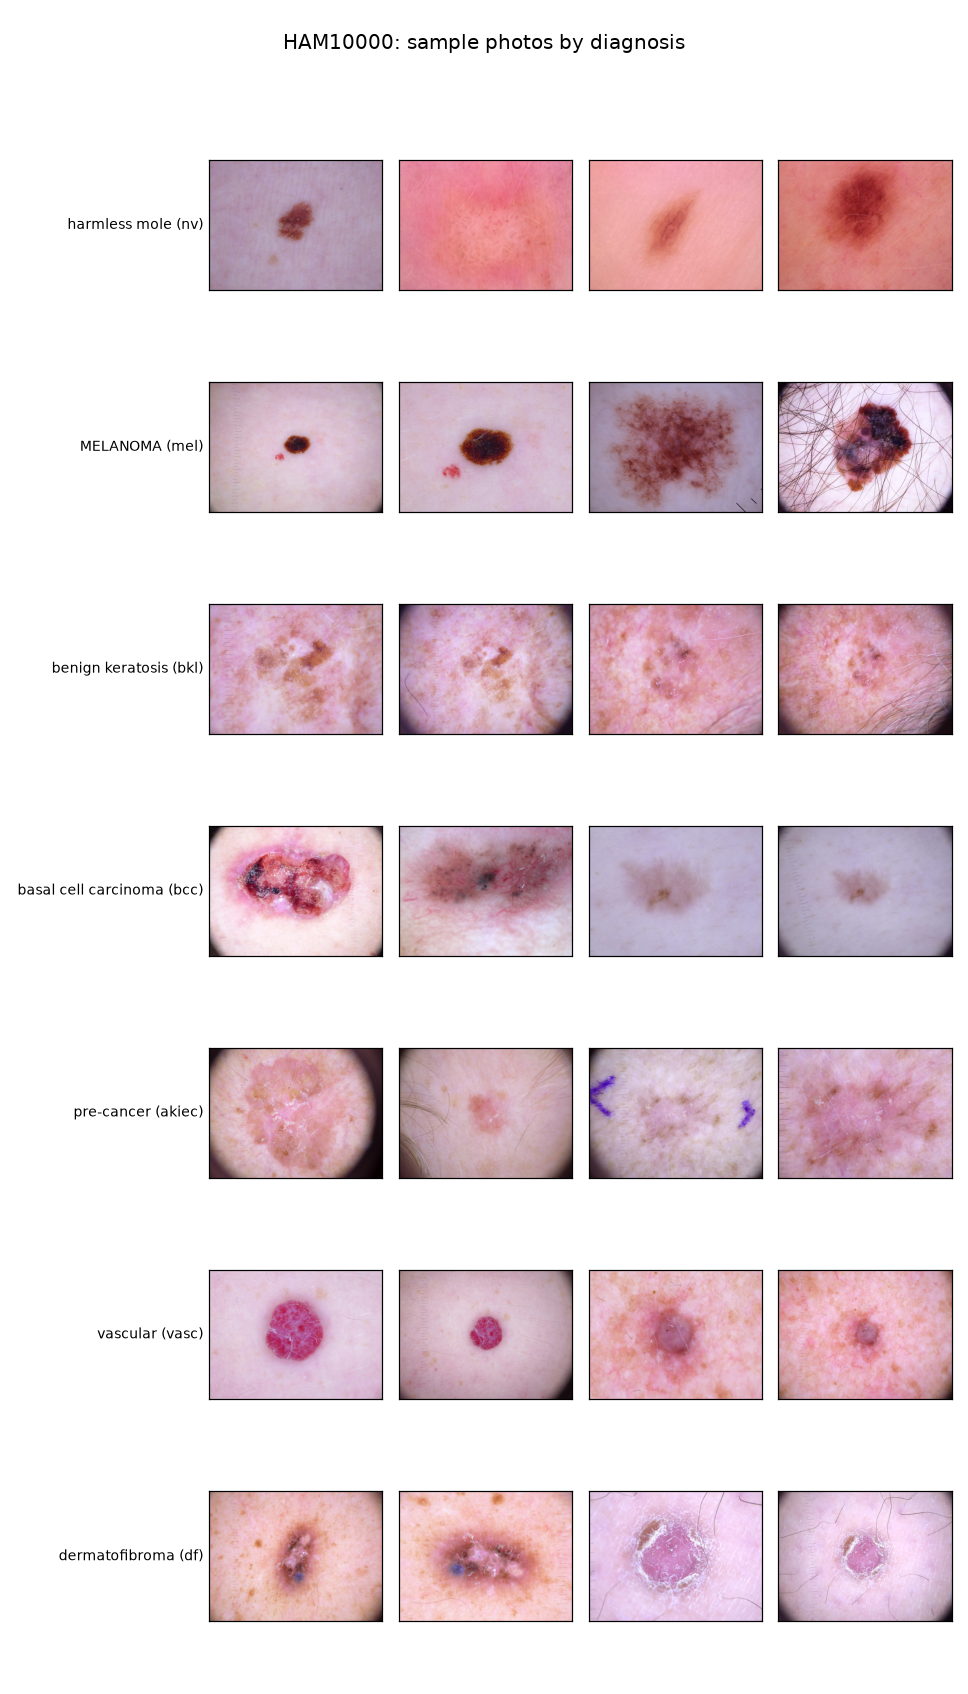
\includegraphics[width=0.9\columnwidth]{figures/sample_photos.png}
\caption{HAM10000 examples, four per class. Clean, magnified, centred---the
easy condition our study degrades.}
\label{fig:samples}
\end{figure}

\section{Methodology}
Fig.~\ref{fig:pipeline} summarises the two pipelines and the evaluation.

\begin{figure}[t]
\centering
\begin{tikzpicture}[
  font=\scriptsize,
  box/.style={draw, rounded corners, align=center, minimum height=6mm, inner sep=2pt},
  >={Stealth[length=1.6mm]}]
\node[box] (img) {Skin image\\(+ optional\\corruption)};
\node[box, above right=2mm and 8mm of img] (enet) {EfficientNet-B0\\(fine-tuned)};
\node[box, below right=2mm and 8mm of img] (dino) {DINOv2\\(frozen)};
\node[box, right=6mm of enet] (soft) {softmax};
\node[box, right=6mm of dino] (knn) {$k$-NN vote\\over library};
\node[box, right=6mm of soft] (co) {label,\\confidence};
\node[box, right=6mm of knn] (cr) {label,\\dist.\ confidence};
\node[box, right=5mm of $(co)!0.5!(cr)$] (ev) {Evaluation:\\bal.\ acc.,\\mel.\ recall,\\ECE, AUROC};
\draw[->] (img) -- (enet); \draw[->] (img) -- (dino);
\draw[->] (enet) -- (soft); \draw[->] (soft) -- (co);
\draw[->] (dino) -- (knn); \draw[->] (knn) -- (cr);
\draw[->] (co) -- (ev); \draw[->] (cr) -- (ev);
\end{tikzpicture}
\caption{The classifier (top) and retrieval (bottom) pipelines share the same
inputs and evaluation.}
\label{fig:pipeline}
\end{figure}

\subsection{Classifier (``Memorizer'')}
An ImageNet-pretrained EfficientNet-B0~\cite{tan2019} with a fresh seven-way head
is fine-tuned with class-weighted cross-entropy to counter imbalance:
\begin{equation}
\mathcal{L} = -\frac{1}{N}\sum_{i=1}^{N} w_{y_i}\,\log p_{i,y_i},
\qquad w_c=\frac{N}{C\,n_c},
\end{equation}
where $p_{i,c}$ is the softmax probability, $n_c$ the count of class $c$, $C{=}7$.
Its confidence is $\max_c p_{i,c}$.

\subsection{Retrieval (``Lookup'')}
Each training image is embedded by a frozen DINOv2 ViT-S/14
($\phi(\cdot)\in\mathbb{R}^{384}$)~\cite{oquab2024} and $L_2$-normalised, forming
a library $\{(\hat\phi_j,y_j)\}$. For a query $q$ with normalised embedding
$\hat\phi_q$, cosine similarity is $s_j=\hat\phi_q^\top\hat\phi_j$. Over the
$k$ nearest neighbours $\mathcal{N}_k(q)$, an inverse-frequency-weighted vote
gives
\begin{equation}
V_c(q)=\frac{1}{n_c}\!\!\sum_{j\in\mathcal{N}_k(q)}\!\! s_j\,\mathbb{1}[y_j=c],
\qquad \hat y=\arg\max_c V_c(q).
\end{equation}
We compare two confidence signals: the winning class's vote share
$V_{\hat y}/\sum_c V_c$, and a \emph{distance} signal
$d(q)=\tfrac{1}{k}\sum_{j\in\mathcal{N}_k(q)} s_j$ mapped to a probability by an
isotonic regressor $g$~\cite{zadrozny2002} fit on a \emph{degraded} validation
set: $\mathrm{conf}(q)=g(d(q))$. Predictions are identical for both signals;
only the confidence differs (Alg.~\ref{alg:ret}).

\begin{algorithm}[t]
\caption{Retrieval classification with distance confidence}
\label{alg:ret}
\begin{algorithmic}[1]
\Require query $q$; library $\{(\hat\phi_j,y_j)\}$; $k$; counts $n_c$; isotonic $g$
\State $\hat\phi_q \gets \phi(q)/\lVert\phi(q)\rVert$
\State $s_j \gets \hat\phi_q^\top\hat\phi_j$ for all $j$;\ \ $\mathcal{N}_k \gets$ top-$k$ by $s_j$
\State $V_c \gets \frac{1}{n_c}\sum_{j\in\mathcal{N}_k} s_j\,\mathbb{1}[y_j{=}c]$;\ \ $\hat y \gets \arg\max_c V_c$
\State $d \gets \frac{1}{k}\sum_{j\in\mathcal{N}_k} s_j$;\ \ $\mathrm{conf}\gets g(d)$
\State \Return $\hat y,\ \mathrm{conf}$
\end{algorithmic}
\end{algorithm}

\subsection{Corruption suite and metrics}
Test images are degraded at three severities for five corruptions---Gaussian
blur, JPEG compression, low light, Gaussian noise, rotation---following the
spirit of~\cite{hendrycks2019}. We report balanced accuracy (mean per-class
recall), melanoma recall, ECE with reliability diagrams~\cite{guo2017,naeini2015},
and OOD AUROC using maximum softmax probability~\cite{hendrycks2017} for the
classifier and mean neighbour similarity for retrieval. ECE is
$\mathrm{ECE}=\sum_{m}\frac{|B_m|}{N}\,\lvert\mathrm{acc}(B_m)-\mathrm{conf}(B_m)\rvert$
over confidence bins $B_m$. All metrics carry bootstrap 95\% confidence
intervals (2{,}000 resamples).

\section{Experimental Setup}
Both models use $224\times224$ inputs and ImageNet normalisation. The classifier
is trained for 5 epochs with AdamW (lr $10^{-4}$), batch size 32, mixed
precision, selecting the best epoch by validation balanced accuracy. Retrieval
uses $k{=}5$ (chosen on validation) and DINOv2 features with no training. The
isotonic calibrator is fit on a degraded 600-image validation subset. Bootstrap
CIs use 2{,}000 resamples. Everything runs on a single laptop GPU (NVIDIA RTX
4050) in PyTorch; code, seeds (42), and the exact lesion-level split are
released for reproducibility.

\section{Results}
\subsection{Clean images}
On clean data the classifier leads (Table~\ref{tab:clean}); a majority-class
baseline (always nv) scores 0.668 accuracy but 0.143 balanced accuracy and zero
melanoma recall, confirming balanced accuracy is the meaningful measure.
Notably, the two models' clean melanoma-recall CIs overlap (0.479--0.629 vs.\
0.401--0.551), so they are \emph{not} significantly different on that class even
on clean images.

\begin{table}[t]
\caption{Clean HAM10000 test set (1{,}502 images), with bootstrap 95\% CIs.}
\label{tab:clean}
\centering
\begin{tabular}{lccc}
\toprule
Model & Accuracy & Balanced acc. & Melanoma recall\\
\midrule
Majority (nv) & 0.668 & 0.143 & 0.000\\
Retrieval     & 0.609 & 0.525\,{\scriptsize[.47,.58]} & 0.473\,{\scriptsize[.40,.55]}\\
Classifier    & \textbf{0.762} & \textbf{0.745}\,{\scriptsize[.70,.79]} & \textbf{0.557}\,{\scriptsize[.48,.63]}\\
\bottomrule
\end{tabular}
\end{table}

\subsection{Degradation: aggregate accuracy hides a melanoma collapse}
Balanced accuracy is mixed (Fig.~\ref{fig:balacc}): the classifier leads under
blur and JPEG but nosedives under low light, noise, and rotation, where
retrieval overtakes it. Melanoma recall (Fig.~\ref{fig:melrec},
Table~\ref{tab:melsevere}) is decisive: the classifier's sensitivity collapses
to near zero under every corruption, while retrieval holds at 34--50\%. Even
under blur and JPEG, where the classifier ``wins'' on aggregate accuracy, it
misses 96--99\% of melanomas.

\begin{table}[t]
\caption{Melanoma recall at the most severe corruption.}
\label{tab:melsevere}
\centering
\begin{tabular}{lcc}
\toprule
Corruption (severe) & Classifier & Retrieval\\
\midrule
Low light & 0.00 & 0.50\\
Noise     & 0.00 & 0.49\\
Blur      & 0.04 & 0.40\\
JPEG      & 0.01 & 0.34\\
Rotation  & 0.08 & 0.50\\
\bottomrule
\end{tabular}
\end{table}

\begin{figure*}[t]
\centering
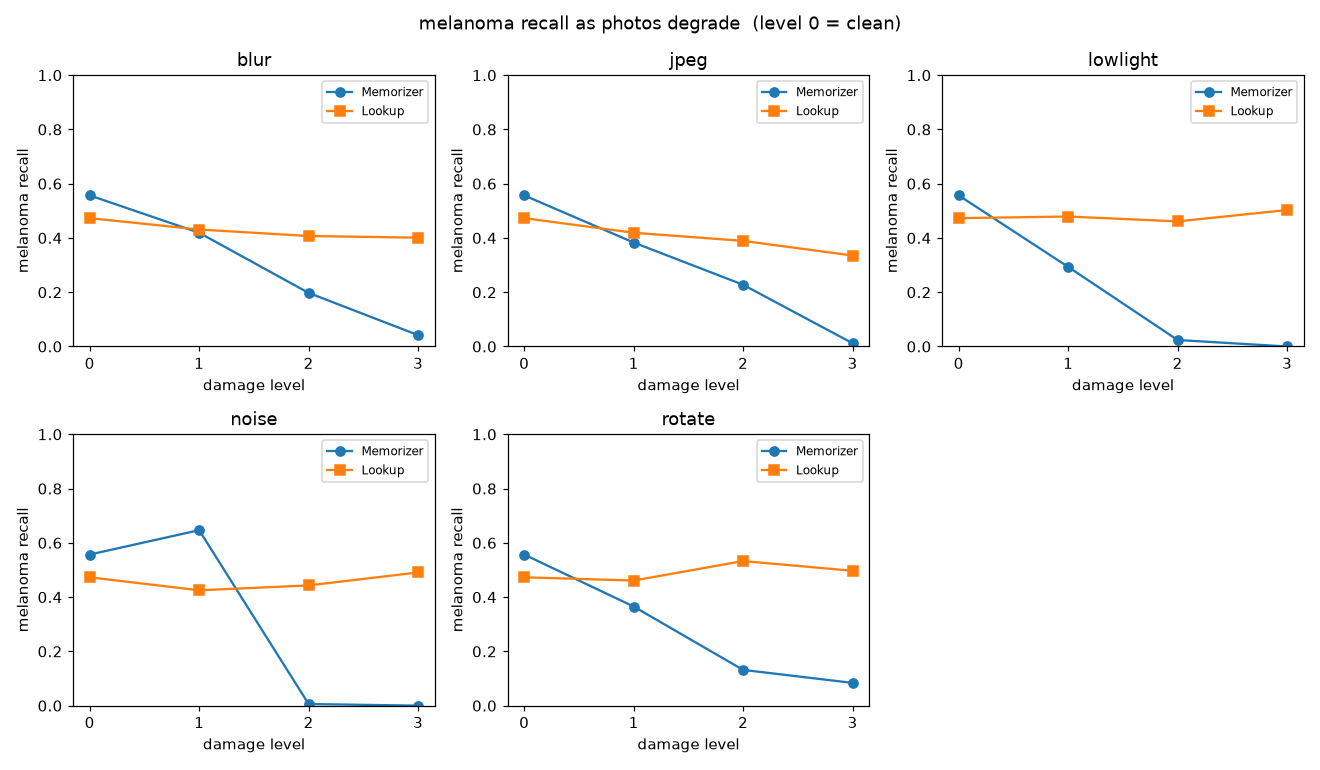
\includegraphics[width=0.9\textwidth]{figures/degradation_melanoma_recall.png}
\caption{Melanoma recall as images degrade (level 0 = clean). The classifier
(blue) collapses toward zero under every corruption; retrieval (orange) stays at
40--50\%. Core robustness result.}
\label{fig:melrec}
\end{figure*}

\begin{figure*}[t]
\centering
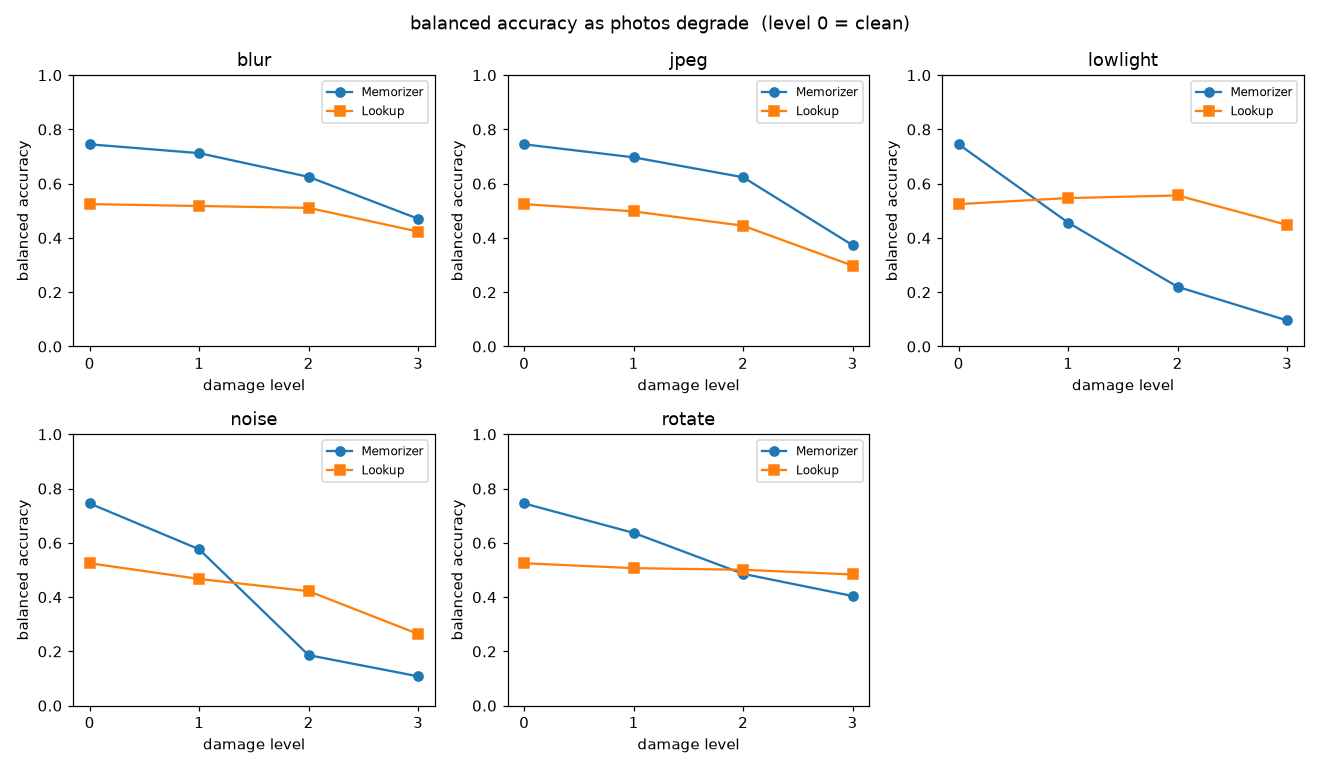
\includegraphics[width=0.9\textwidth]{figures/degradation_balanced_accuracy.png}
\caption{Balanced accuracy as images degrade. Retrieval overtakes the classifier
under low light, noise, and rotation; the classifier leads under blur and
JPEG---an honestly mixed aggregate picture.}
\label{fig:balacc}
\end{figure*}

\subsection{Calibration and ablation of the confidence signal}
Table~\ref{tab:ece} ablates the retrieval confidence signal against the
classifier. Vote share is badly overconfident and worsens under corruption;
the distance signal, calibrated on degraded validation data, is the best
calibrated and \emph{improves} under corruption (Fig.~\ref{fig:reliab}). A
neighbour-count ablation on validation balanced accuracy gives 0.379, 0.513,
0.511, 0.511, 0.508 for $k{=}1,5,9,15,25$; we use $k{=}5$.

\begin{table}[t]
\caption{Ablation: expected calibration error (lower = more honest).}
\label{tab:ece}
\centering
\begin{tabular}{lcc}
\toprule
Confidence signal & Clean & Heavily degraded\\
\midrule
Classifier softmax        & 0.08 & 0.14\\
Retrieval, vote share     & 0.23 & 0.31\\
Retrieval, distance (ours)& \textbf{0.05} & \textbf{0.03}\\
\bottomrule
\end{tabular}
\end{table}

\begin{figure}[t]
\centering
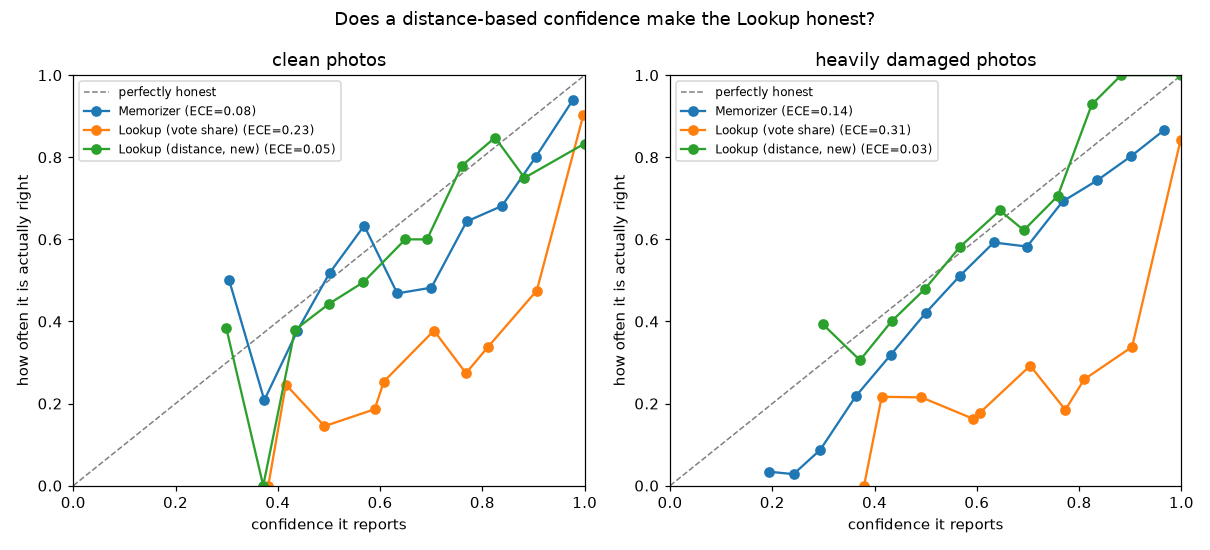
\includegraphics[width=\columnwidth]{figures/calibration_lookup_reliability.png}
\caption{Reliability diagrams (clean vs.\ heavily degraded). The distance-based
retrieval confidence (green) hugs the diagonal; vote share (orange) sits far
below it.}
\label{fig:reliab}
\end{figure}

\subsection{An honest negative: selective prediction}
Allowing abstention on the least-confident inputs raises overall accuracy on the
retained set, and the classifier's softmax triages overall accuracy \emph{better}
than retrieval's distance confidence. However, abstention does \emph{not} raise
melanoma recall for retrieval (it stays near 0.45 on degraded images at all
referral rates): a globally well-calibrated score is not necessarily a good
per-error ranking signal. We report this rather than omit it.

\subsection{Real-world smartphone photos}
On PAD-UFES-20 (no retraining) both models lose accuracy---expected for a
dermoscopy-to-smartphone shift (Table~\ref{tab:pad}). Yet retrieval catches
$3.5\times$ more melanomas (0.404 vs.\ 0.115, non-overlapping CIs), and its
similarity signal separates familiar HAM from unfamiliar PAD at AUROC 0.937
(CI 0.929--0.945) versus 0.720 (0.704--0.738) for the classifier's softmax,
which stays confident on data it cannot handle (Fig.~\ref{fig:ood}).

\begin{table}[t]
\caption{Real smartphone photos (PAD-UFES-20, 2{,}106 images), 95\% CIs.}
\label{tab:pad}
\centering
\begin{tabular}{lccc}
\toprule
Model & Accuracy & Melanoma recall & OOD AUROC\\
\midrule
Classifier & 0.290 & 0.115\,{\scriptsize[.04,.21]} & 0.720\,{\scriptsize[.70,.74]}\\
Retrieval  & 0.273 & \textbf{0.404}\,{\scriptsize[.27,.54]} & \textbf{0.937}\,{\scriptsize[.93,.95]}\\
\bottomrule
\end{tabular}
\end{table}

\begin{figure*}[t]
\centering
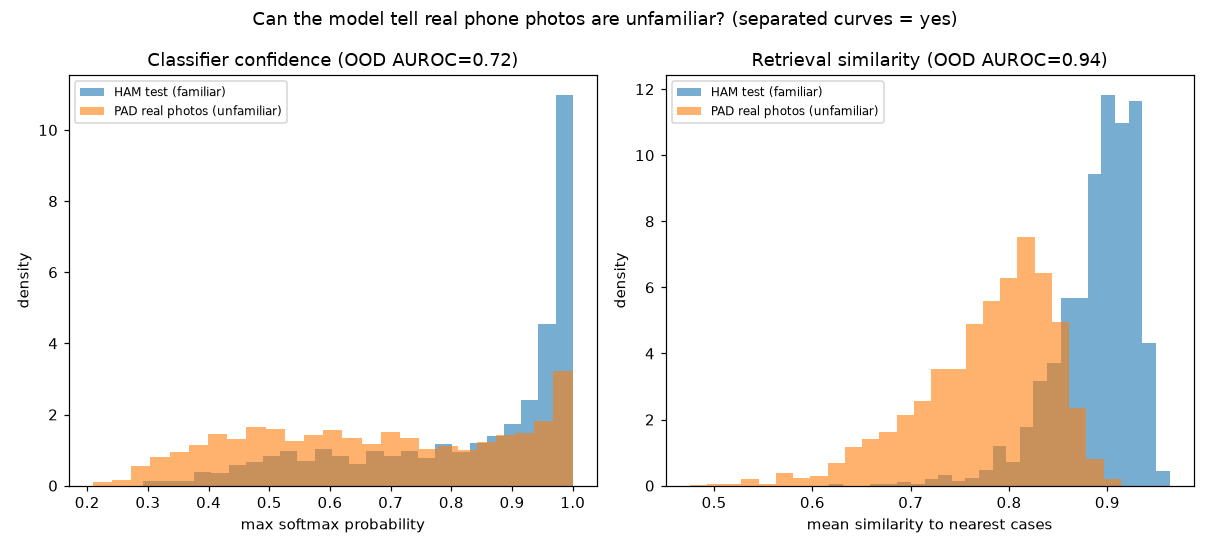
\includegraphics[width=0.9\textwidth]{figures/pad_ood_detection.png}
\caption{Familiar (HAM, blue) vs.\ unfamiliar (real PAD, orange) signal
distributions. The classifier confidence (left) overlaps and stays high on both;
retrieval similarity (right) separates them (AUROC 0.94).}
\label{fig:ood}
\end{figure*}

\subsection{Error analysis}
Fig.~\ref{fig:neigh} shows, for melanoma queries, the five nearest stored cases
the retrieval model consults. Correct cases sit beside other melanomas; missed
cases sit beside benign look-alikes (nevi, dermatofibroma, actinic keratosis)
that are hard for clinicians too. This case-based transparency, unavailable to a
classifier, both explains predictions and localises failure.

\begin{figure*}[t]
\centering
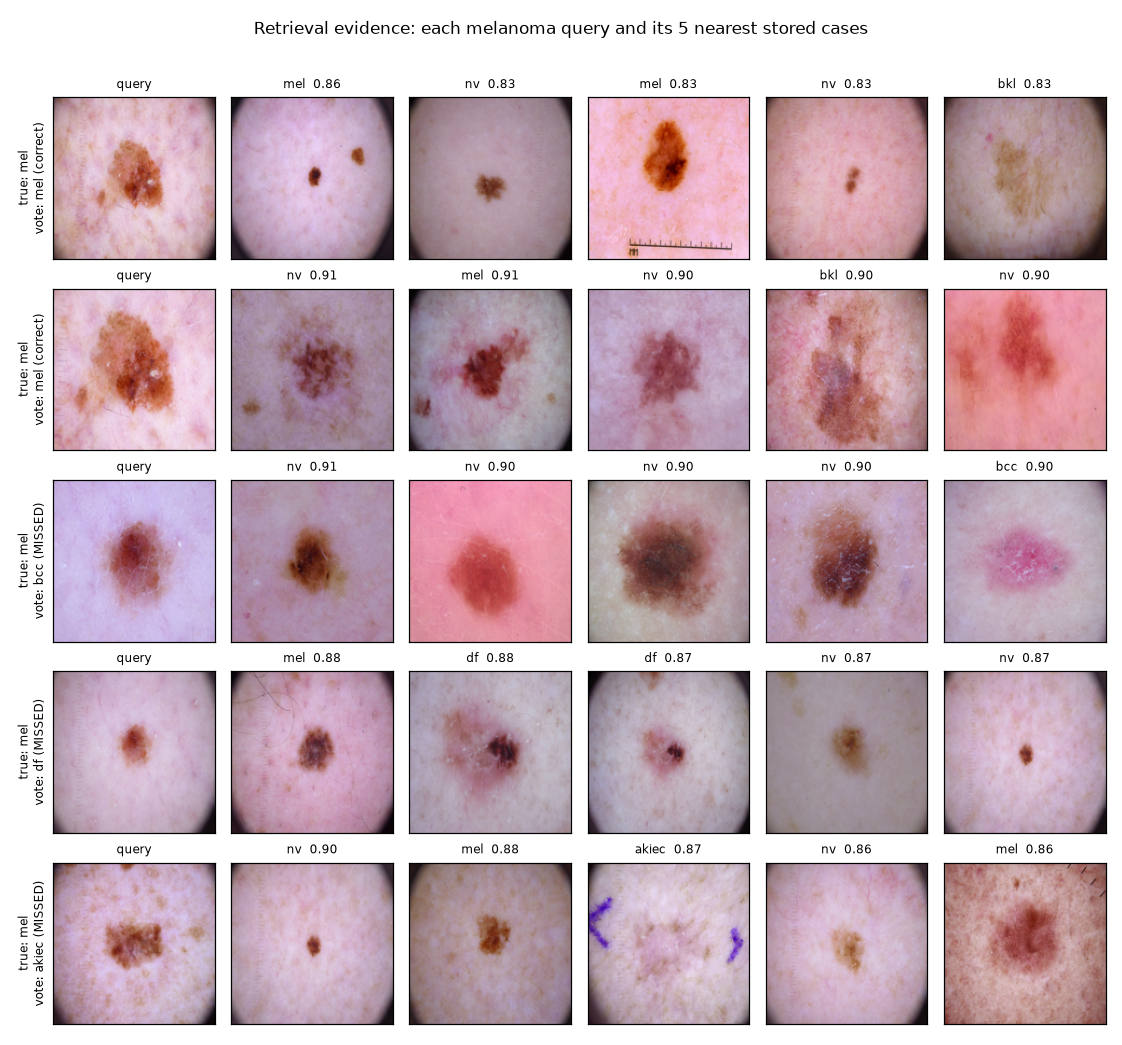
\includegraphics[width=0.86\textwidth]{figures/retrieval_neighbours.png}
\caption{Retrieval evidence: each melanoma query with its five nearest stored
cases (label and cosine similarity). Rows 1--2 are voted correctly; rows 3--5
are missed, surrounded by benign look-alikes.}
\label{fig:neigh}
\end{figure*}

\section{Discussion}
The results argue for judging screening models by \emph{trust} rather than
clean-set accuracy. A classifier that is more accurate on curated data can fail
silently and catastrophically on the malignant class under realistic
degradation, remaining confident throughout. Retrieval trades some clean-image
accuracy for two deployment-relevant properties: graceful degradation of
melanoma sensitivity, and---given a distance-based confidence---honest
uncertainty that survives distribution shift and flags unfamiliar inputs. The
calibration finding is methodological: for retrieval the confidence
\emph{definition} determines honesty under shift. The selective-prediction
negative refines this: calibration improves the \emph{value} of a confidence
score without necessarily improving its \emph{ranking} of likely errors.

\section{Limitations}
The controlled corruptions are simulated, though we mitigate this with a real
smartphone dataset. Training uses a single source (HAM10000); the
dermoscopy-to-macroscopic shift is large, so absolute accuracy on PAD is low for
both models and neither is a deployable product. The retrieval fingerprint is a
general (not skin-specific) embedding, and the study was single-GPU and
short. Reference details should be verified before formal submission.

\section{Conclusion and Future Work}
On degraded and real-world skin images, a retrieval model with a distance-based,
shift-calibrated confidence is simultaneously more robust on melanoma and more
honest about its uncertainty than a strong classifier, whereas aggregate
accuracy hides the classifier's silent melanoma failures. Future work: a
skin-specific foundation embedding (e.g., PanDerm~\cite{yan2025panderm} or
BiomedCLIP~\cite{zhang2025biomedclip}); fairness across skin tones (PAD-UFES-20
provides Fitzpatrick labels); error-aware referral signals beyond global
calibration; and additional real-world datasets.

\section*{Reproducibility}
Code, the exact lesion-level split, trained-model configuration, corruption
definitions, and all evaluation scripts are available at
\url{https://github.com/nishankhareln/skin_research}.

\begin{thebibliography}{00}
\bibitem{esteva2017} A. Esteva \emph{et al.}, ``Dermatologist-level classification of skin cancer with deep neural networks,'' \emph{Nature}, vol. 542, pp. 115--118, 2017.
\bibitem{tschandl2018} P. Tschandl, C. Rosendahl, and H. Kittler, ``The HAM10000 dataset, a large collection of multi-source dermatoscopic images of common pigmented skin lesions,'' \emph{Sci. Data}, vol. 5, 180161, 2018.
\bibitem{pacheco2020} A. G. C. Pacheco \emph{et al.}, ``PAD-UFES-20: A skin lesion dataset composed of patient data and clinical images collected from smartphones,'' \emph{Data in Brief}, vol. 32, 106221, 2020.
\bibitem{codella2018} N. C. F. Codella \emph{et al.}, ``Skin lesion analysis toward melanoma detection: A challenge at ISIC,'' in \emph{Proc. IEEE ISBI}, 2018.
\bibitem{tan2019} M. Tan and Q. Le, ``EfficientNet: Rethinking model scaling for convolutional neural networks,'' in \emph{Proc. ICML}, 2019.
\bibitem{oquab2024dinov2} M. Oquab \emph{et al.}, ``DINOv2: Learning robust visual features without supervision,'' \emph{Trans. Mach. Learn. Res. (TMLR)}, 2024.
\bibitem{zhang2025biomedclip} S. Zhang \emph{et al.}, ``BiomedCLIP: A multimodal biomedical foundation model trained from fifteen million image--text pairs,'' \emph{NEJM AI}, vol. 2, no. 1, 2025, doi: 10.1056/AIoa2400640.
\bibitem{yan2025panderm} S. Yan \emph{et al.}, ``A multimodal vision foundation model for clinical dermatology,'' \emph{Nat. Med.}, vol. 31, no. 8, pp. 2691--2702, 2025, doi: 10.1038/s41591-025-03747-y.
\bibitem{hendrycks2019} D. Hendrycks and T. Dietterich, ``Benchmarking neural network robustness to common corruptions and perturbations,'' in \emph{Proc. ICLR}, 2019.
\bibitem{maron2021} R. C. Maron \emph{et al.}, ``A benchmark for neural network robustness in skin cancer classification,'' \emph{Eur. J. Cancer}, vol. 155, pp. 191--199, 2021.
\bibitem{hu2024diffusion} M. Hu \emph{et al.}, ``Diffusion model driven test-time image adaptation for robust skin lesion classification,'' \emph{arXiv:2405.11289}, 2024.
\bibitem{bissoto2022artifact} A. Bissoto, C. Barata, E. Valle, and S. Avila, ``Artifact-based domain generalization of skin lesion models,'' in \emph{Proc. ECCV Workshops (ISIC)}, 2022.
\bibitem{disalvo2024medmnistc} F. Di Salvo, S. Doerrich, and C. Ledig, ``MedMNIST-C: Comprehensive benchmark and improved classifier robustness by simulating realistic image corruptions,'' in \emph{Proc. MICCAI Workshop (ADSMI)}, 2024.
\bibitem{guo2017} C. Guo, G. Pleiss, Y. Sun, and K. Q. Weinberger, ``On calibration of modern neural networks,'' in \emph{Proc. ICML}, 2017.
\bibitem{naeini2015} M. P. Naeini, G. Cooper, and M. Hauskrecht, ``Obtaining well calibrated probabilities using Bayesian binning,'' in \emph{Proc. AAAI}, 2015.
\bibitem{zadrozny2002} B. Zadrozny and C. Elkan, ``Transforming classifier scores into accurate multiclass probability estimates,'' in \emph{Proc. ACM KDD}, 2002.
\bibitem{fayyad2024conformal} J. Fayyad, S. Alijani, and H. Najjaran, ``Empirical validation of conformal prediction for trustworthy skin lesions classification,'' \emph{Comput. Methods Programs Biomed.}, vol. 253, 108231, 2024.
\bibitem{penso2024calibration} C. Penso, L. Frenkel, and J. Goldberger, ``Confidence calibration of a medical imaging classification system that is robust to label noise,'' \emph{IEEE Trans. Med. Imag.}, vol. 43, no. 6, pp. 2050--2060, 2024.
\bibitem{sambyal2023understanding} A. S. Sambyal, U. Niyaz, N. C. Krishnan, and D. R. Bathula, ``Understanding calibration of deep neural networks for medical image classification,'' \emph{Comput. Methods Programs Biomed.}, vol. 242, 107816, 2023.
\bibitem{gassner2023secbir} M. Gassner \emph{et al.}, ``Saliency-enhanced content-based image retrieval for diagnosis support in dermatology consultation: Reader study,'' \emph{JMIR Dermatology}, vol. 6, e42129, 2023.
\bibitem{gupta2023mednn} D. Gupta, R. Loane, S. Gayen, and D. Demner-Fushman, ``Medical image retrieval via nearest neighbor search on pre-trained image features,'' \emph{Knowledge-Based Systems}, vol. 278, 110907, 2023.
\bibitem{he2022demal} X. He, Y. Wang, S. Zhao, and X. Chen, ``Deep metric attention learning for skin lesion classification in dermoscopy images,'' \emph{Complex Intell. Syst.}, vol. 8, no. 2, pp. 1487--1504, 2022.
\bibitem{hendrycks2017} D. Hendrycks and K. Gimpel, ``A baseline for detecting misclassified and out-of-distribution examples in neural networks,'' in \emph{Proc. ICLR}, 2017.
\bibitem{zimmerer2022mood} D. Zimmerer \emph{et al.}, ``MOOD 2020: A public benchmark for out-of-distribution detection and localization on medical images,'' \emph{IEEE Trans. Med. Imag.}, vol. 41, no. 10, 2022.
\bibitem{gutbrod2025openmibood} M. Gutbrod, D. Rauber, D. W. Nunes, and C. Palm, ``OpenMIBOOD: Open medical imaging benchmarks for out-of-distribution detection,'' in \emph{Proc. IEEE/CVF CVPR}, 2025.
\bibitem{huang2022multiscale} Z. Huang, T. Wang, Y. Cai, and L. Liang, ``A multi-scale framework for out-of-distribution detection in dermoscopic images,'' in \emph{Proc. ML4CS}, 2022.
\bibitem{abhishek2025dermamnist} K. Abhishek, A. Jain, and G. Hamarneh, ``Investigating the quality of DermaMNIST and Fitzpatrick17k dermatological image datasets,'' \emph{Sci. Data}, vol. 12, no. 1, 196, 2025.
\bibitem{geifman2017} Y. Geifman and R. El-Yaniv, ``Selective classification for deep neural networks,'' in \emph{Proc. NeurIPS}, 2017.
\bibitem{liu2022ldu} J. Liu, B. Gallego, and S. Barbieri, ``Incorporating uncertainty in learning to defer algorithms for safe computer-aided diagnosis,'' \emph{Sci. Rep.}, vol. 12, 1762, 2022.
\bibitem{verma2023multiexpert} R. Verma, D. Barrej\'{o}n, and E. Nalisnick, ``Learning to defer to multiple experts: Consistent surrogate losses, confidence calibration, and conformal ensembles,'' in \emph{Proc. AISTATS}, 2023.
\bibitem{dvijotham2023codoc} K. Dvijotham \emph{et al.}, ``Enhancing the reliability and accuracy of AI-enabled diagnosis via complementarity-driven deferral to clinicians,'' \emph{Nat. Med.}, vol. 29, no. 7, 2023.
\end{thebibliography}

\end{document}
